\subsection{Noise}

% (TODO): Write about main motivation for doing this: what if we have a model
% e.g. in software that we are now implementing physically: how does the model
% then respond to the noise?

% (TODO): Find some more background information on previous works, both in general
% and with ESN in particular. What is the contribution of this work at all?

A comparison can be drawn to commonly recommended SNRs in the IEEE 802.11
standard for Wi-Fi communications, ranging from 15db to 25dB. Below this
threshold, wireless communication will quickly become unusable.

In summary, our results indicate a robustness to the presence of noise in the
input stream. This is a promising result when considering physical substrates as
reservoir mediums, providing lower bounds on the ratio of signal power to noise
power that is necessary.

\subsection{Measurement equipment accuracy}

In Fig. \ref{adc_quantization} we see a performance degradation from 3000 to
1000 discernible states, something of which is more pressing for the bigger
reservoirs. As discrete output states move beneath 1000, the performance quickly
deteriorates. However, even with just 10 discrete outputs, reservoirs are still
able to replicate the input sequence to some degree. Furthermore, reservoirs
with 400 hidden nodes and just 100 discrete output bins consistently provide the
same performance as that of a reservoir with 50 hidden nodes and no output
quantization.

A 12-bit ADC has $2^{12}$, or 4096 output codes, which in accordance with our
experiments would impose no noticeable increase in the prediction error. 16-bit
ADCs, outputting $2^{16}$, or 65536 discrete states, would influence our ESN
simulations even less. In \cite{soriano_delay-based_2015}, a major factor
limiting performance of a nonlinear analog electric circuit implementation was
quantization noise. Low error rates on the Mackey-Glass task were achieved with
8 bits or more in the ADC. This result is also seen in our ESN implementation,
where NRMSE starts leveling out around 8 bits of accuracy, or 256 discrete
states.

These results demonstrate that the reservoir methodology provides an inherent
resilience to output quantization. When designing physical RC systems, this may
be applied in preliminary analysis of the output resolution and representation,
whether it be voltage in electrode arrays or the magnetic polarization of
permalloy nanomagnets.

% (TODO): I don't really like the conclusion here -- could I conclude with
% something more _concrete_, almost like tricks of the trade?

\subsection{Partially observable reservoir state}

When attaching input units to the network by weights, experience has shown that
choosing $\mathbf{W}_{in}$ can be done freely, as long as
$\rho(\mathbf{W}_{res}) < 1$ is satisfied \cite{jaeger_echo_2001}. Experimental
results from adjusting the sparsity of $\mathbf{W}_{in}$ is shown in
Fig. \ref{partial_visibility}a, in which all experiments were done with a
uniform input weight distribution in the interval [-0.5, 0.5].

Across all three reservoir sizes, we see a small increase in the signal
prediction error when increasing input connectivity from an initial density of
0.1. While finding the optimal reservoir perturbance clearly depends on the
memory capacity and computational dynamics required for the task at hand, this
benchmark task gives a clear indication of the influence of input sparsity in
general. The relatively low sensitivity to this parameter suggests that physical
reservoirs may achieve excellent performance even when only perturbing selected
parts of the system. An input stream parameter found to be of greater relevance
is input scaling, i.e. the amplitude of the input signal that the reservoir sees
\cite{alippi_quantification_2009}. The necessary scaling depends on the
nonlinearity needed, as inputs far from 0 drive $\tanh$ neurons towards
saturation. In a physical reservoir design setting, this parameter is often
possible to adjust after-the-fact, as opposed to changing the physical hardware
layout of the system.

Next, a general trend seen when adjusting output connectivity, is a slight,
linear decrease in performance from a completely dense output matrix to a
density of 0.4 (Fig. \ref{partial_visibility}b). Furthermore, for the 50 and 100
node reservoirs, there is a noticeable transition from a linear to an
exponential NRMSE growth.

We may understand these results to indicate that there is a critical point in
the output density space where there the readout layer starts seeing enough of
the reservoir dynamics to reconstruct the input NARMA10 signal. Additionally,
when the output density exceeds this threshold, the performance will continue to
grow linearly with the density, achieving the best performance at full
connectivity.

% (TODO): Also plot output connectivity as amount of output nodes. Perhaps we see
% that the size of the underlying reservoir does not matter at all?

In \cite{jensen_computation_2018}, artificial spin ice is explored as a
substrate for physical RC. Here, nanomagnetic assemblies are perturbed, using an
external magnetic field as input source. Thus, every magnet sees exactly the
same input stream.

Fig. \ref{input_scaling_distrib} explores the performance of ESNs with three
different input weight distributions: uniform, Gaussian and fixed. Despite the
performance disparity with increasing input scaling, the best performance of all
three classes hover around the same NRMSE of around 0.25. This demonstration of
scaling differently distributed inputs such that they all achieve acceptable
performance bodes well for physical RC. In particular, we observe a promising
result when considering RC with physical substrates in which every node is
forced to receive the same input.

% (TODO): Ensure that the subfigure figure isn't pushed _into_ the references.

\subsection{Topology}

Topology section. Probably a literature review, leading into discussions about
future work.

\begin{figure}[H]
  \centering
  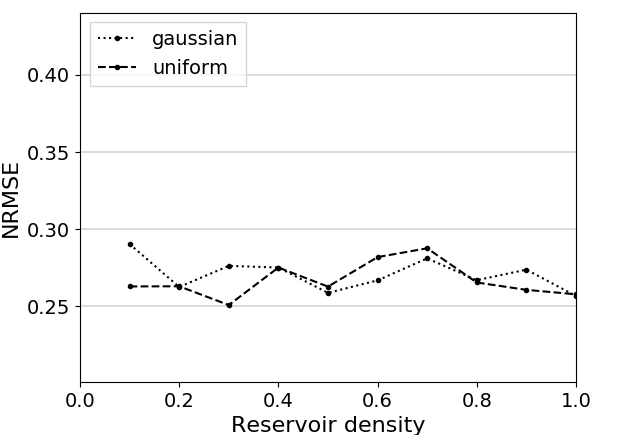
\includegraphics[width=2.5in]{img/reservoir_density_distrib.png}
  \caption{
    Reservoir density versus for two weight distributions. Fixed weight will not
work for internal nodes, unless special topology is employed, e.g. ring
(elaborate). This shows that sparse internal weight matrices work fine.
  }
  \label{reservoir_density_distrib}
\end{figure}

Something about internal reservoir density as an introductory exploration.

% (TODO): Reason for reservoir sparsity is in the original Jaeger paper,
% e.g. multiple creating separate networks with rich dynamics.

%%% Local Variables:
%%% mode: latex
%%% TeX-master: "../main"
%%% End:
